% !TeX spellcheck = en_GB
%%%%%%%%%%%%%%%%%%%%%%%%%%%%%%%%%%%%%%%%%%
%                                        %
%    Engineer thesis LaTeX template      % 
%                                        %
%%%%%%%%%%%%%%%%%%%%%%%%%%%%%%%%%%%%%%%%%%



\documentclass[a4paper,twoside,12pt]{book}
\usepackage[utf8]{inputenc}                                      
\usepackage[T1]{fontenc}  
\usepackage{amsmath,amsfonts,amssymb,amsthm}
\usepackage[polish,british]{babel} 
\usepackage{indentfirst}
\usepackage{lmodern}
\usepackage{graphicx} 
\usepackage{hyperref}
\usepackage{booktabs}
\usepackage{tikz}
\usepackage{pgfplots}
\usepackage{mathtools}
\usepackage{geometry}
\usepackage[page]{appendix} 

\usepackage{setspace}
\onehalfspacing


\frenchspacing

\usepackage{listings}
\lstset{
	language={},
	basicstyle=\ttfamily,
	keywordstyle=\lst@ifdisplaystyle\color{blue}\fi,
	commentstyle=\color{gray}
}

%%%%%%%%%

 

%%%%%%%%%%%% FANCY HEADERS %%%%%%%%%%%%%%%

\usepackage{fancyhdr}
\pagestyle{fancy}
\fancyhf{}
\fancyhead[LO]{\nouppercase{\it\rightmark}}
\fancyhead[RE]{\nouppercase{\it\leftmark}}
\fancyhead[LE,RO]{\it\thepage}


\fancypagestyle{onlyPageNumbers}{%
   \fancyhf{} 
   \fancyhead[LE,RO]{\it\thepage}
}

\fancypagestyle{PageNumbersChapterTitles}{%
   \fancyhf{} 
   \fancyhead[LO]{\nouppercase{\it\rightmark}}
   \fancyhead[RE]{\nouppercase{\it\leftmark}}
   \fancyhead[LE,RO]{\it\thepage}
}


%%%%%%%%%%%%%%%%%%%%%%%%%%%
% listings 
\usepackage{listings}
\lstset{%
language=C++,%
commentstyle=\textit,%
identifierstyle=\textsf,%
keywordstyle=\sffamily\bfseries, %\texttt, %
%captionpos=b,%
tabsize=3,%
frame=lines,%
numbers=left,%
numberstyle=\tiny,%
numbersep=5pt,%
breaklines=true,%
morekeywords={descriptor_gaussian,descriptor,partition,fcm_possibilistic,dataset,my_exception,exception,std,vector},%
escapeinside={@*}{*@},%
%texcl=true, % wylacza tryb verbatim w komentarzach jednolinijkowych
}
%%%%%%%%%%%%%%%%%%%%%%%%%%%%%%%%%%%%

%%%% TODO LIST GENERATOR %%%%%%%%%

\usepackage{color}
\definecolor{brickred}      {cmyk}{0   , 0.89, 0.94, 0.28}

\makeatletter \newcommand \kslistofremarks{\section*{Remarks} \@starttoc{rks}}
  \newcommand\l@uwagas[2]
    {\par\noindent \textbf{#2:} %\parbox{10cm}
{#1}\par} \makeatother


\newcommand{\ksremark}[1]{%
{%\marginpar{\textdbend}
{\color{brickred}{[\foreignlanguage{polish}{#1}]}}}%
\addcontentsline{rks}{uwagas}{\protect{\foreignlanguage{polish}{#1}}}%
}

%%%%%%%%%%%%%% END OF TODO LIST GENERATOR %%%%%%%%%%% 

% some issues...

\newcounter{PagesWithoutNumbers}

\newcommand{\hcancel}[1]{%
    \tikz[baseline=(tocancel.base)]{
        \node[inner sep=0pt,outer sep=0pt] (tocancel) {#1};
        \draw[red] (tocancel.south west) -- (tocancel.north east);
    }%
}%

\newcommand{\MonthName}{%
  \ifcase\the\month
  \or January% 1
  \or February% 2
  \or March% 3
  \or April% 4
  \or May% 5
  \or June% 6
  \or July% 7
  \or August% 8
  \or September% 9
  \or October% 10
  \or November% 11
  \or December% 12
  \fi}


%%%%%%%%%%%%%%%%%%%%%%%%%%%%%%%%%%%%%%%%%%%%%%
% Helvetica font macros for the title page:
\newcommand{\headerfont}{\fontfamily{phv}\fontsize{18}{18}\bfseries\scshape\selectfont}
\newcommand{\titlefont}{\fontfamily{phv}\fontsize{18}{18}\selectfont}
\newcommand{\otherfont}{\fontfamily{phv}\fontsize{14}{14}\selectfont}

%%%%%%%%%%%%%%%%%%%%%%%%%%%%%%%%%%%%%%%%%%%%%%
%%%%%%%%%%%%%%%%%%%%%%%%%%%%%%%%%%%%%%%%%%%%%%
%%%%%%%%%%%%%%%%%%%%%%%%%%%%%%%%%%%%%%%%%%%%%%
%%%%%%%%%%%%%%%%%%%%%%%%%%%%%%%%%%%%%%%%%%%%%%
%%%%%%%%%%%%%%%%%%%%%%%%%%%%%%%%%%%%%%%%%%%%%%
%%%%%%%%%%%%%%%%%%%%%%%%%%%%%%%%%%%%%%%%%%%%%%
%%%%%%%%%%%%%%%%%%%%%%%%%%%%%%%%%%%%%%%%%%%%%%


\newcommand{\Author}{Wojciech Drzewiecki}
\newcommand{\Supervisor}{Krzysztof Simiński, PhD DSc}
\newcommand{\Consultant}{Name Surname, PhD}
\newcommand{\Title}{Central online voting system}
\newcommand{\Polsl}{Silesian University of Technology}
\newcommand{\Faculty}{Faculty of Automatic Control, Electronics, and Computer Science}



\begin{document} 

\kslistofremarks

\cleardoublepage
	
%%%%%%%%%%%%%%%%%%  Title page %%%%%%%%%%%%%%%%%%% 
\pagestyle{empty}
{
	\newgeometry{top=2.5cm,%
	             bottom=2.5cm,%
	             left=3cm,
	             right=2.5cm}
	\sffamily
	\rule{0cm}{0cm}
	
	\begin{center}
	
\includegraphics[width=29mm]{polsl}
	\end{center} 
	\vspace{1cm}
	\begin{center}
	\headerfont \Polsl
	\end{center}
	\begin{center}
	\headerfont \Faculty
	\end{center}
	\vfill
	\begin{center}
	\titlefont Engineer thesis
	\end{center}
	\vfill
	
	\begin{center}
	\otherfont \Title\par
	\end{center}
	
	\vfill
	
	\vfill
	 
	\noindent\vbox
	{
		\hbox{\otherfont author: \Author}
		\vspace{12pt}
		\hbox{\otherfont supervisor: \Supervisor}
		% \vspace{12pt}
		% \hbox{\otherfont consultant: \Consultant}
	}
	\vfill 
 
   \begin{center}
   \otherfont Gliwice,  \MonthName\ \the\year
   \end{center}	
	\restoregeometry
}
  

\cleardoublepage
 

\rmfamily
\normalfont


%%%%%%%%%%%% statements required by law and Dean's office %%%%%%%%%%
\cleardoublepage

\begin{flushright}
załącznik nr 2 do zarz. nr 97/08/09 
\end{flushright}

\vfill  

\begin{center}
\Large\bfseries Oświadczenie
\end{center}

\vfill

\foreignlanguage{polish}{Wyrażam  zgodę / Nie wyrażam zgody*  na  udostępnienie  mojej  pracy  dyplomowej / rozprawy doktorskiej*.}

\vfill

Gliwice, dnia {\selectlanguage{polish}\today}

\vfill

\rule{0.5\textwidth}{0cm}\dotfill 

\rule{0.5\textwidth}{0cm}
\begin{minipage}{0.45\textwidth}
{\begin{center}(podpis)\end{center}}
\end{minipage} 

\vfill

\rule{0.5\textwidth}{0cm}\dotfill 

\rule{0.5\textwidth}{0cm}
\begin{minipage}{0.45\textwidth}
{\begin{center}\rule{0mm}{5mm}(poświadczenie wiarygodności podpisu przez Dziekanat)\end{center}}
\end{minipage}


\vfill

* podkreślić właściwe

 


%%%%%%%%%%%%%%%%%%%%%  
\cleardoublepage

\rule{1cm}{0cm}

\vfill  

\begin{center}
\Large\bfseries Oświadczenie promotora
\end{center}

\vfill

\foreignlanguage{polish}{Oświadczam, że praca „\Title” spełnia wymagania formalne pracy dyplomowej inżynierskiej.}

\vfill



\vfill

Gliwice, dnia {\selectlanguage{polish}\today}

\rule{0.5\textwidth}{0cm}\dotfill 

\rule{0.5\textwidth}{0cm}
\begin{minipage}{0.45\textwidth}
{\begin{center}(podpis promotora)\end{center}}
\end{minipage} 

\vfill
 
 

\cleardoublepage


%%%%%%%%%%%%%%%%%% Table of contents %%%%%%%%%%%%%%%%%%%%%%
\pagenumbering{Roman}
\pagestyle{onlyPageNumbers}
\tableofcontents

%%%%%%%%%%%%%%%%%%%%%%%%%%%%%%%%%%%%%%%%%%%%%%%%%%%%%
\setcounter{PagesWithoutNumbers}{\value{page}}
\mainmatter
\pagestyle{PageNumbersChapterTitles}

%%%%%%%%%%%%%% body of the thesis %%%%%%%%%%%%%%%%%


\chapter{Introduction}



\chapter{Online voting systems}

\section{Introduction}

	Ever since internet was introduced in our lives, online election voting was a contentious issue.

	First of all, online voting would be convenient---right now voting is associated with going to a nearby ward, waiting in a queue, 
	complicated procedure of receiving a ballot and filling a ballot.
	Moreover, waiting for results could be decreased---now we have to wait for all the votes to be counted, protocols sent to commissions,
	summed up, and determination of the winners. All this can take over few dozen hours.
	Online voting would decrease that time hugely, at the same time being much more precise than counting by a person.
	
	On the other hand, there is significant trust issue. There will always be a person which have access to data, 
	and with such access that person could change elections results in a matter of seconds.
	Following this lead, even if nobody has access to data, we will never be sure that vote we cast is not changed somewhere in the logic of the application.
	We can eliminate that by developing open source application, which can be verified that it does not change something in the logic.
	This approach would create many more problems, of which two are: firstly, open source application can be investigated by everyone, 
	and with given source it is much easier to find a hole in the logic from which we can benefit.
	Secondly, even if we see view of that open source application, we can never be sure that logic behind it is not swapped.
	
	You can see a pattern here---for every argument there is a counter argument, which generates another problems. 
	There is no right answer in this debate.

\section{Ideal voting system}

  So what would be features of the perfect voting system? Let's investigate it along with flow of online voting.

  Before election, system administrator has to enter committees and candidates data into a system, register them for polls predicted for certain date, which he have \ksremark{(Nie jestem rodowitym użytkownikiem angielszczyzny, zatem moje uwagi językowe proszę brać z rezerwą) has} entered at the beginning.
  Although he could handle registering candidates to certain committees, he cannot handle scope of managing whole committee during election. 
  It's best if administrator granted some chosen user privileges to manage certain committee inside the system---let's call him committee administrator.
  It's useful for example in case of allocation seats via D'Hondt method---it's committee itself that wants to decide on order in closed list, there should be no third party involved.
  
  First, in order to cast a vote through internet, a citizen would have to register. What online voting system wants to achieve is for citizens \ksremark{for citizens is} to be able to cast a vote without leaving home.
  It makes sense that citizens would register also through the internet---for example in case of some injury, if someone could go out of home, they could also vote in a ward. 
  It creates a problem---how do we know that person on the other side of the screen is who he says he is. 
  Solution is two step authentication process---citizen registers with citizen id (for example PESEL in Poland), he is sent a text message or an email,
  but also receives registered letter of registration, both with activation codes, that only together allows him to register properly. 
  Registered letter allows to verify citizen willing to vote through internet without need of leaving the house. 
  Because email can be generated without interference of any third party person, code sent this way secures citizen from someone taking advantage of code in letter.
  Those two ways combined secure citizens account from being taken advantage of.

  Let's say a citizen registered successfully. On election day, he should be able to vote on exactly the same polls as he would personally, in ward.
  Citizen should be able to cast a vote only once, and his vote should be detached from his account---in no way should anybody be able to tell which vote belongs to which citizen.
  Although registered for online voting, a citizen should still be able to vote personally in ward. 
  However, once he voted in any of two ways, the second one should be automatically and immediately blocked. This requires for the system to work also in wards.
  Once user votes online or receives a ballot from commission in a ward, he should be immediately blocked for second type of voting.

  Citizen easily and securely voted either through internet or personally. Now his journey ends, he can go back to living his life. 
  What's left to do is to calculate results of election. However, system also has to take into account all votes casted in wards.
  Results can be calculated if and only if all wards have entered their protocols into the system.
  To do so, a member of a commission should be assigned with access to send the protocol to the system---let's call him a ward administrator. 
  Once that member is a registered user, he should be able to be assigned as particular ward admin by the system administrator.
  Then, he should be able to file in the protocol, once the election is closed for voting.
  
  After closing the election and collecting protocols from all wards, results of the election can be calculated.
  This information can be public and delivered to public on the same site that they voted on, as well as on official government electoral commission website.

\section{Overview of similar solutions}

  \subsection{Electronic voting in Estonia}
    In Estonia, voting is based on electronic citizen ID. It's mandatory and sufficient national identity document, which allows for secure remote authentication.
    To cast a vote, an Estonian needs a computer connected to the internet and equipped with card reader.
    They can authenticate using digital certificate included in their citizen card, and cast a vote on the internet \cite{bib:internet_voting_estonia}. \ksremark{Trochę inaczej się cytuje – poprawiłem w pliku \texttt{thesis.bib}. Wpisy bibliograficzne w Bib\TeX u są zwykle dostępne w internecie.}

    This solution is problematic for several reasons:
    \begin{itemize}
      \item It's impossible to be easily implemented in countries without electronic citizen ID. 
        Providing such documents for most of society of the country is a long time process, measured in years rather than months.
      \item A card reader capable of reading such a card is not a common device---a citizen has to go somewhere with a card reader, if he wants to cast a vote.
      \item Electronic citizen ID is not an intellectual knowledge like password or token. 
        It's a physical device that can be easily stolen---and of course blocked in some department---but it may be too late and someone may have already taken advantage from owning someone else's citizen ID.
    \end{itemize}

\chapter{Requirements and tools}

  \section{Functional requirements}
  \ksremark{Zdanie wprowadzające – może być jedna linijka.}
    \begin{itemize}
      \item A citizen of a country that holds an online election in the application should be able to register.
      \item The application should allow registered citizens to vote on candidates of their preference.
      \item A vote of a citizen should be taken into account when calculating results of an election.
      \item A citizen should be able to cast only one vote per election.
      \item A vote of a citizen should not be trackable---no person should be able to tell which citizen voted on which candidate.
      \item A person designated as a ward administrator---and only that person---should be able to send a ward protocol to the system.
      \item Protocols sent from wards should be taken into account when calculating results of an election.
      \item A person designated as a commission administrator---and only that person---should be able to enter a commission's closed list candidates order to the system.
      \item An administrator of the application should be able to perform steps that lead to creation of an election identical to one provided to him.
      \item An administrator should be able to trigger calculation of the results of an election.
      \item Election results should not be calculated with some of ward protocols missing.
      \item An administrator should be able to grant privileges of ward and commission administrators to designated people separately.
      \item An administrator should not be able to perform actions in replacement of  a ward or committee administrator.
    \end{itemize}

  \section{Nonfunctional requirements}
  \ksremark{Zdanie wprowadzające – może być jedna linijka.}
    \begin{itemize}
      \item User interface should be understandable to English speaking individuals.
      \item The application should be implemented in Java, with help of Spring Boot and related frameworks for an backend, 
      and Thymeleaf template engine for an frontend.
      \item The application should store all necessary data in a MySQL database.
      \item The application should hash all sensitive data stored in a database.
      \item The application should offer all available functionalities on Google Chrome version 79.
    \end{itemize}
  \pagebreak

  \section{Use cases}
    \subsection{Citizen use case UML}
    \begin{figure}[h]
      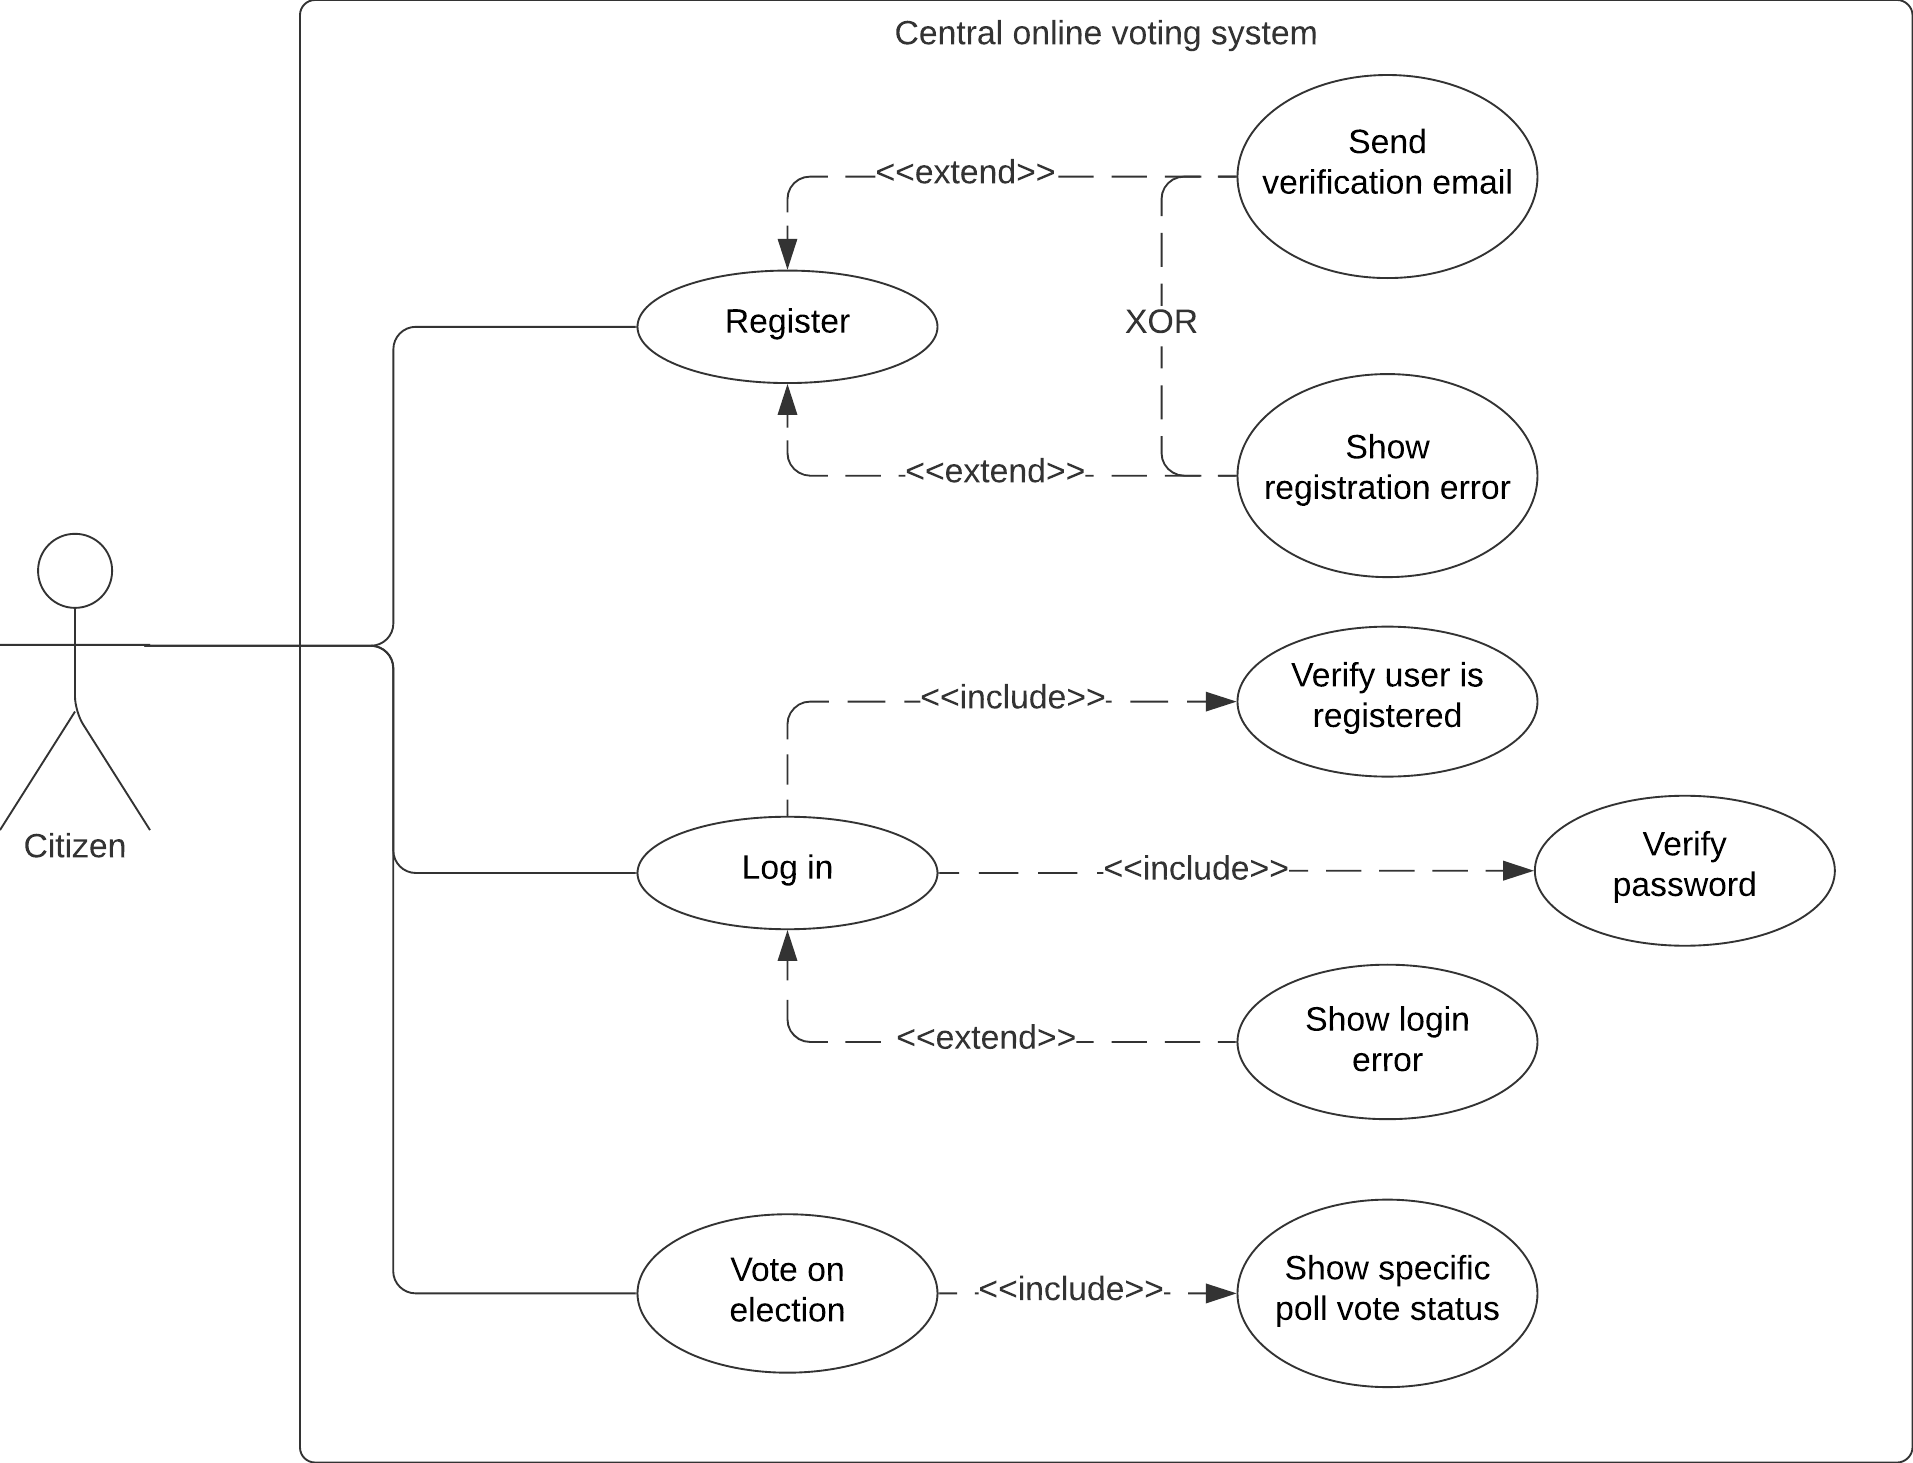
\includegraphics[width=\linewidth]{citizen_uml.png}
      \caption{Citizen use case UML for \Title}
      \label{fig:citizen_uml}
    \end{figure}

    Figure \ref{fig:citizen_uml} shows available use cases for a citizen. He can register and in that case he will receive an email, 
    or he can see some error regarding registration. A citizen can try to login, which will trigger checks if he is registered and that password matches.
    In case of any errors, he will see a message. 
    A citizen can vote, and after that he will see status of his vote regarding every poll in the election, no matter if vote is valid or not.
    \ksremark{Czy użytkownik, który się jeszcze nie zalogował «citizen» może głosować?}
    \pagebreak

    \subsection{Ward administrator use case UML}
    \begin{figure}[h]
      \centering
      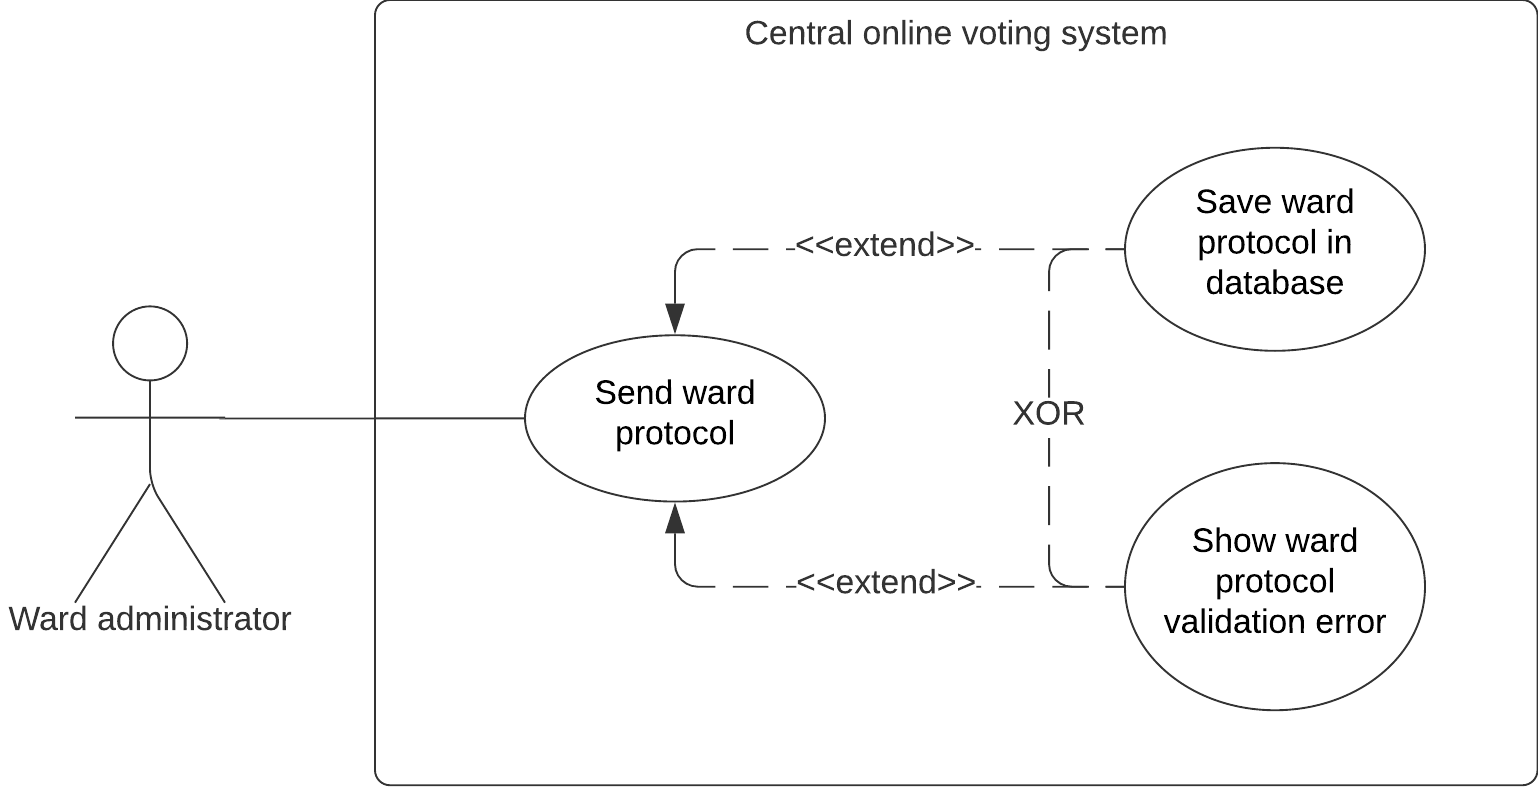
\includegraphics[width=0.65\linewidth]{ward_admin_uml.png}
      \caption{Ward administrator use case UML for \Title}
      \label{fig:ward_admin_uml}
    \end{figure}

    Figure \ref{fig:ward_admin_uml} shows available use cases for a ward administrator. A ward administrator can try to send a ward protocol.
    If anything is not correct in a protocol he tried to send, he will see a validation error, and the protocol will not be sent.

    \subsection{Committee administrator use case UML}
    \begin{figure}[h]
      \centering
      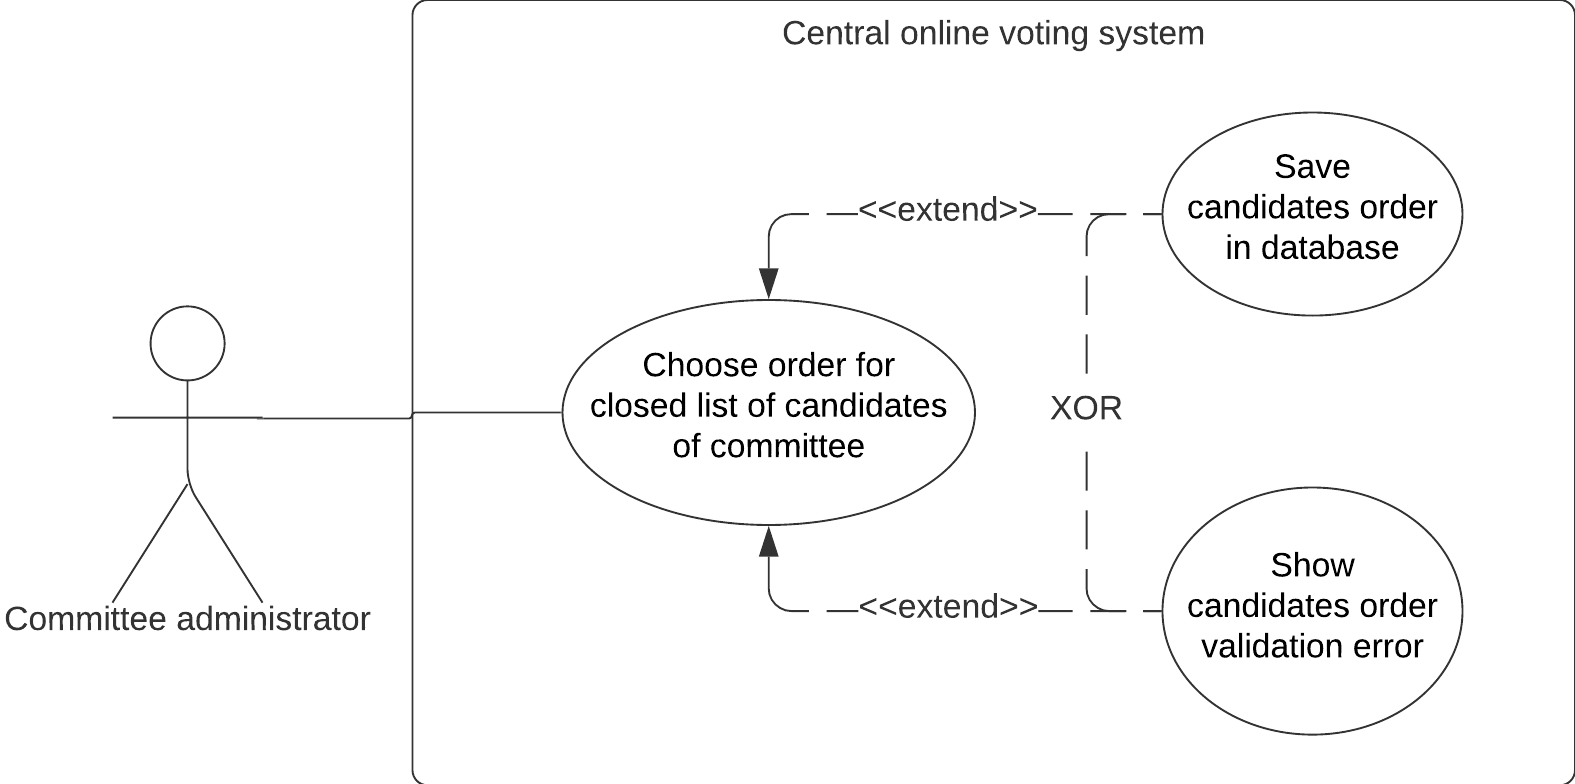
\includegraphics[width=0.65\linewidth]{committee_admin_uml.png}
      \caption{Committee administrator use case UML for \Title}
      \label{fig:committee_admin_uml}
    \end{figure}

    Figure \ref{fig:committee_admin_uml} shows available use cases for a committee administrator. A committee administrator can send closed list candidates' order.
    If anything is not correct in an order of candidates, he will see a validation error, and the candidates order will not be saved.
    \pagebreak

    \subsection{Administrator use case UML}
    \begin{figure}[h]
      \centering
      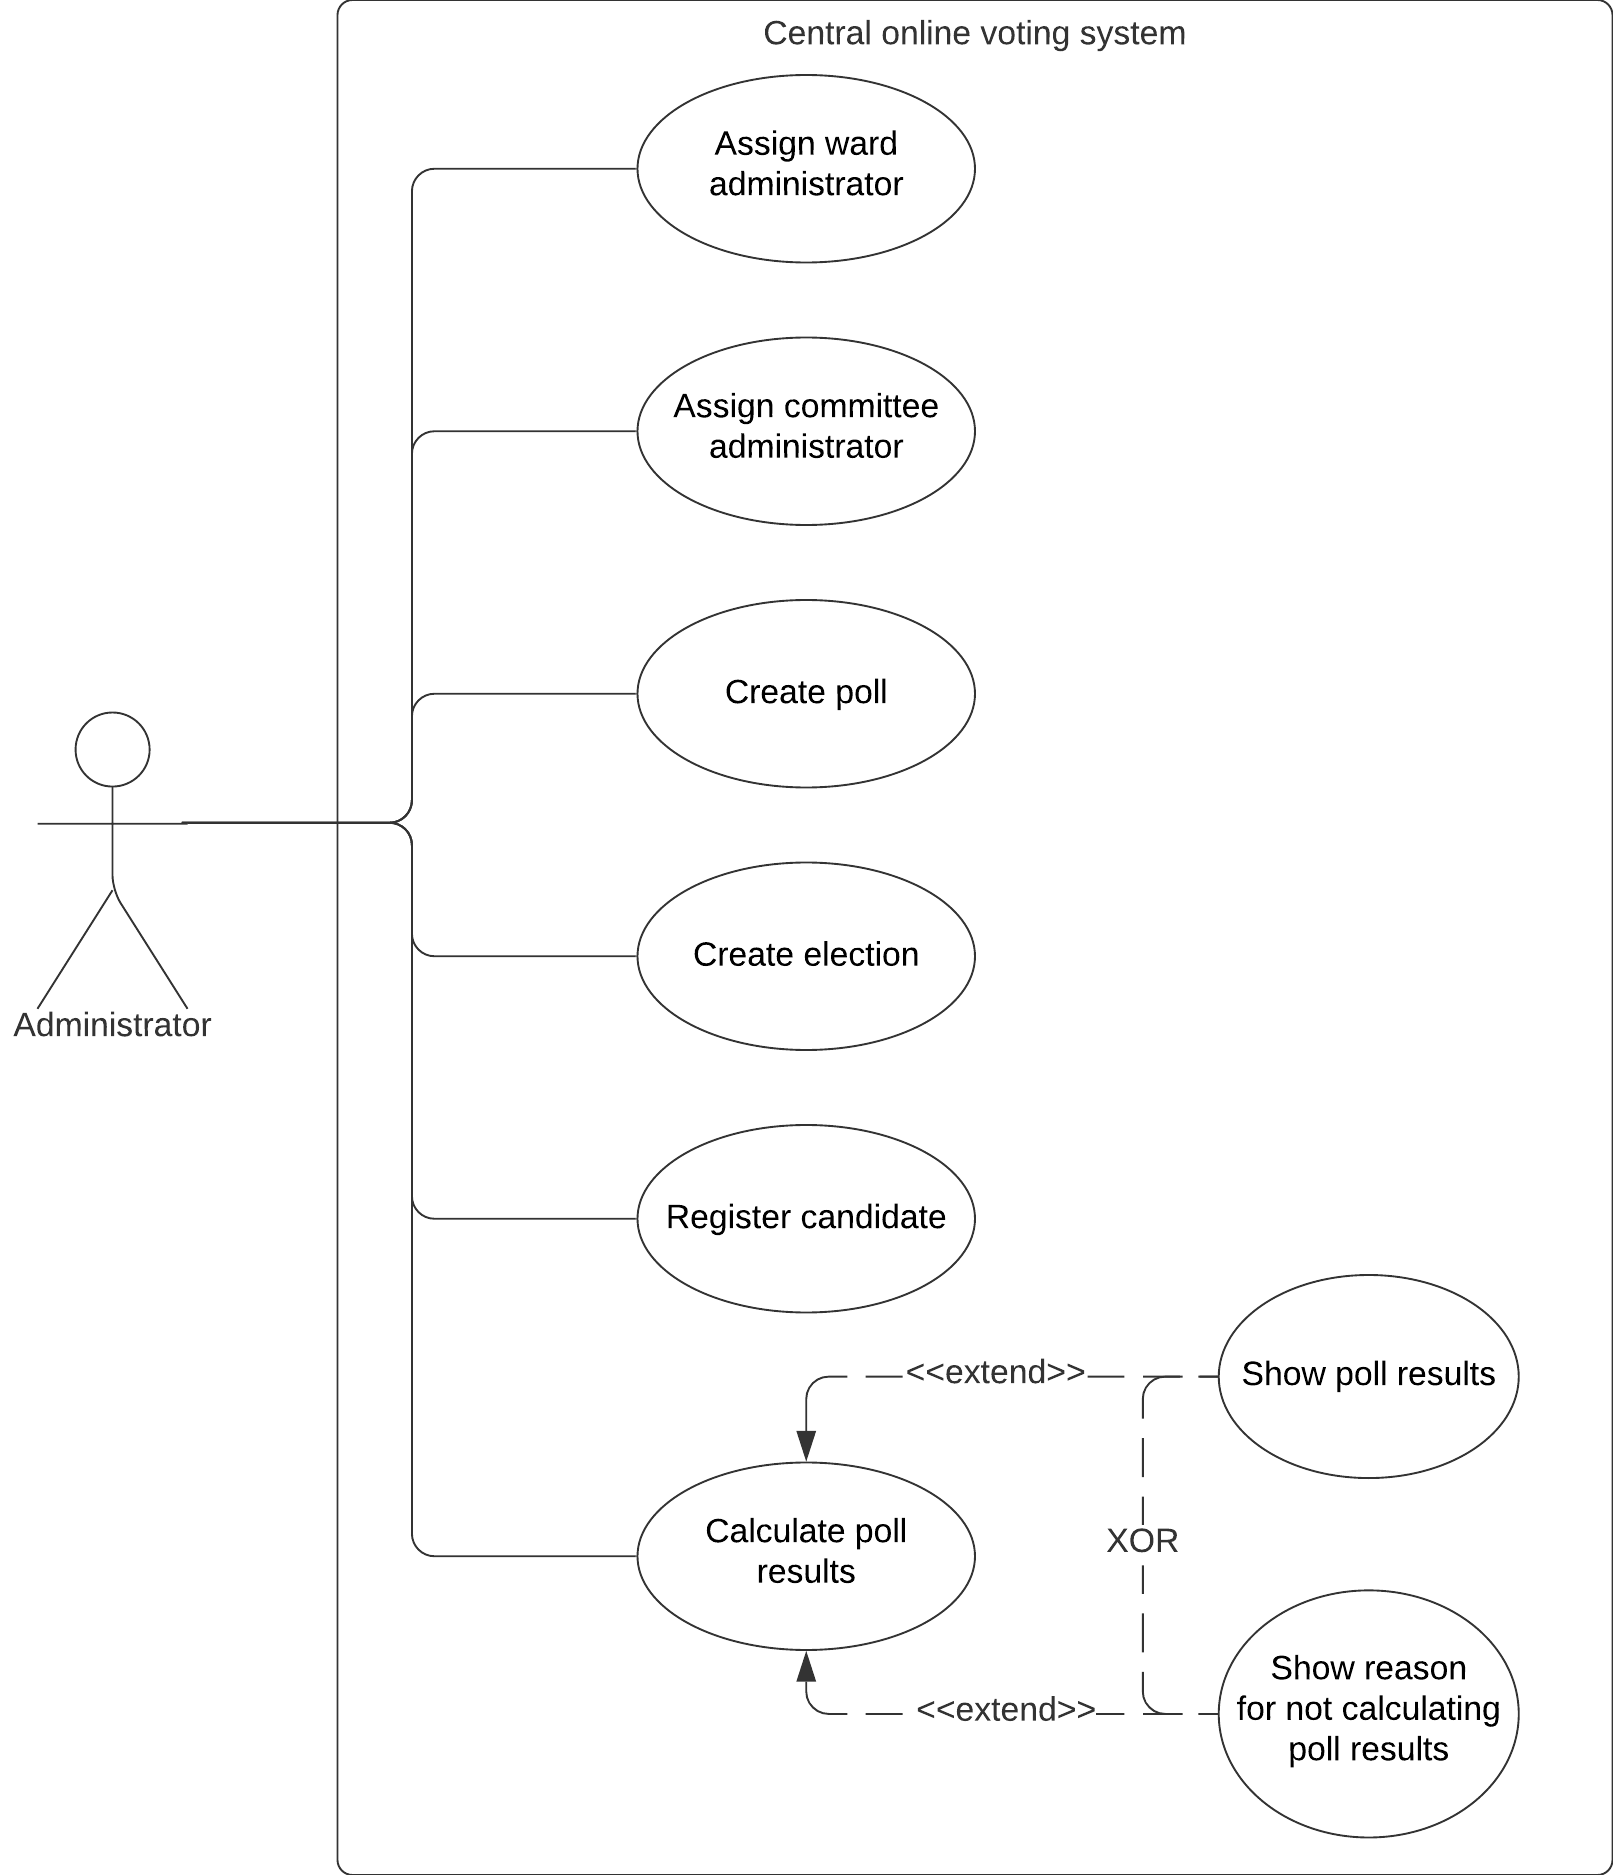
\includegraphics[width=0.8\linewidth]{admin_uml.png}
      \caption{Administrator use case UML for \Title}
      \label{fig:admin_uml}
    \end{figure}

    Figure \ref{fig:admin_uml} shows available use cases for an administrator. We assume that an administrator knows what he is doing, so there is no need to validate his choices.
    However, he has no power over how many protocols are sent from wards when he wants to calculate poll results. 
    Thus he will get appropriate message when he tries to calculate results of poll that is not ready to be calculated.

  \section{Description of tools}
    The application is developed in Java programming language with Spring Framework and Thymeleaf as template engine. 
    Data is stored in a MySQL database, and whole application is built with  Apache Maven build automation tool.

    \subsection{Java}
      It's \ksremark{It is} an object--oriented programming language that requires Java Virtual Machine to run a program. 
      This allows Java applications to run on almost every device, regardless of it's operational system\cite{bib:horstmann2008core}.
      Java offers huge open--source ecosystem.

      \subsubsection{Alternative}
        C\# is also an object--oriented programming language, but it's \ksremark{it is} used to develop software for Microsoft platforms\ksremark{spacja przed cytowaniem}\cite{bib:thai2003net}.

      Although there is no much difference in beginner level development between Java and C\#, I find C\# less convenient than Java,
      because I use machine with macOS operating system as my everyday work tool, and Java has huge support on Unix based system, compared to almost none support for C\#.

    \subsection{Maven}
      Apache Maven is a tool that is capable of building and managing any Java-based project. 
      It helps developers with dependency management, as it's able to download all necessary dependencies with almost no participation of developer.
      It's easy for beginners, as it's build lifecycles and syntax is easy to understand---all You need is artifact info of dependency that You want to include in Your project, 
      and it will download and include dependency in project during install build lifecycle\cite{bib:maven}.

      \subsubsection{Alternatives}
        \paragraph{Gradle}
          It's also application build tool for Java-based projects. It's better than Maven for larger projects, thanks to better automation methods and better performance.
          Gradle is built with more experienced and demanding developer in mind\cite{bib:gradle}. \ksremark{odstęp między słowej a cytowaniem}
        
        \paragraph{Ant}
          Ant is a powerful tool that allows developer to automate very complicated task, but this functionality is not cheap.
          It's complicated to configure and it's being ousted by Gradle\cite{bib:ant}.

      \paragraph{} %I know it's probably not the way to achieve this result, but it works
      I chose Maven because I wanted to learn modern build technology that is common in the industry, but is suitable for beginners.

    \subsection{Spring}
      It's an open--source framework for Java platform. It focuses on delivering out--of--the--box core features for any kind of application, 
      so developers can focus on business logic of the application. 
      Aside from Spring Core, which provides easy dependency injection, Spring provides extensions in form of more or less independent modules, each available as it's own maven artifact.\cite{bib:spring} \ksremark{Cytowanie przed kropką.}
      Spring Boot is an extension of Spring framework, which provides out--of--the--box configuration, and requires user to provide only application specific configuration.
      
      \subsubsection{Alternative}
        Because Spring is open--source framework, considered a standard in the industry for over 10 years, there is no other framework that is as feature--packed as Spring.
        One could make a case for .Net framework for C\# language, but it's \ksremark{it is} developed and directed by Microsoft\cite{bib:thai2003net}, 
        whereas Spring is powered by community, and contains features required by that same community. 

      \subsubsection{Spring Security}
        Authentication and Authorization framework for Spring based applications. Provides quick protection of API exposed by application and
        integration with users in database. Allows for assigning users' roles, and managing accesses based on these roles\cite{bib:spring_security}.

      \subsubsection{Spring Web MVC}
        It's designed around front controller pattern, and helps developers follow the Model--View--Controller design pattern.
        It coordinates flow of request processing performed by configurable delegate components\cite{bib:spring_web_mvc}.
      
      \subsubsection{Spring Data JPA}
        Spring implementation of JPA contract, powered by Hibernate. Reduces hugely boilerplate code that's associated with querying database,
        especially with Repository interface custom finder methods\cite{bib:spring_data_jpa}.

    \subsection{Thymeleaf}
      Modern server-side Java template engine resolver. 
      It converts HTML files with Thymeleaf--specific dynamic attributes based on model attributes provided by developer through Spring MVC framework\cite{bib:thymeleaf}.
      
      \subsubsection{Alternative}
        There are not many pure alternatives when it comes to template resolvers. 
        Java Enterprise Edition comes with JSP, which is not pleasant to use, and is considered obsolete.
        It definitely does not provide level of integration with Spring MVC framework as much as Thymeleaf does.

  \section{Methodology of design and implementation}
    Base of every application is a well designed database schema. 
    Once schema is considered with required functionalities of application in mind, and with space for extensibility predicted,
    it makes development not only go faster and more efficient, but also more pleasant for a developer.

    With proper database schema, we have to consider what is the best way for user to use our application---through web browser or application?
    Because application is meant to be nation--wide, 
    and there is a web browser on perhaps every computer with internet connection---which is necessary for application to work---web application is the way to go.
    
    When designing web application, we have to decide how we want to achieve end result---presenting view to application user.
    There are two most common approaches when it comes to Spring application:
    \begin{itemize}
      \item Exposing REST API from Spring application, that contains all of business logic and create another application, that consumes that API and interacts with the user in any way desired.
      \item Keep view rendering on server side, and expose pure html to the user.
    \end{itemize}
    I chose the second option, because it is not the most important thing for \Title\ to be pretty and responsive, I wanted to focus on backend side of the application.

    Once view presenting is established, we want to consider how we want to design architecture of the application.
    I can see two approaches in choosing the architecture: basing on application requirements or basing on technology used in application.
    Because Spring provides whole framework dedicated to MVC design pattern, and also it's widely used in the industry, I chose to develop application in that manner,
    rather than choosing architecture basing on application requirements. 
    My application is not large enough to be hugely impacted by bad architecture. I could only harm my project by using some fancy architecture.

\chapter{External specification}
  \section{Types of users and cockpits}
    \subsection{Overview}
    In order to secure application from unauthorized access  I divided application into four main cockpits:
    \begin{itemize}
      \item Voter cockpit
      \item Administrator cockpit
      \item Ward administrator cockpit
      \item Committee administrator cockpit
    \end{itemize}
    Each cockpit has certain role that is necessary to even display available actions \ksremark{?}. 
    In order to have access to anything we have to be authenticated (active, successfully registered) user, with assigned role that gives us permission for certain cockpits.
    A guest---not registered user---is only available to register or login.

    \subsection{Voter cockpit}
    A user with a role of a voter is able to vote for election and see election results after it's \ksremark{it is} closed.
    In case of voting a user is be able to vote on a poll only once without any exception.

    \subsection{Administrator cockpit}
    A user with a role of an administrator is able to create essential data---wards, polls, committees etc. as well as granting certain roles to certain users.
    An administrator is not be able to interfere in a ward or committee administration other than choosing its administrator.
    Moreover administrator is the one that triggers polls results calculation.

    \subsection{Ward administrator cockpit}
    A user with a role of a ward administrator is able to manage only his assigned ward. Under no circumstances he is able to manage other wards.
    In a ward administrator cockpit he is able to enter a  protocol from a ward for each poll during an election.

    \subsection{Committee administrator cockpit}
    A user with a role of a committee administrator is able to manage only his assigned committee. Under no circumstances he is able to manage other committees.
    In a committee administrator cockpit he is able to choose an order of committee candidates in a closed list. 
  
  \section{Software requirements}
    %TODO: Add database installed piece
    In order to run the application, You \ksremark{you} have to have Java 12, Maven 3.6.X installed on Your \ksremark{your} computer, 
    make sure that \lstinline[language=bash]|java| and \lstinline[language=bash]|mvn| executables are in PATH environment variable.

  \section{Installation procedure}
    %TODO: Add database connection procedure
    In order to build project, we \ksremark{W poprzedniej sekcji analogiczny opis korzystał z <<you>>, ten z <<we>>.} have to execute Maven install lifecycle \lstinline[language=bash]|mvn install| in APP\_ROOT directory.
    This lifecycle will generate \lstinline[language=bash]|ballotbox-0.0.1-SNAPSHOT.jar| jar file in APP\_ROOT/target directory.
    To run application we just have to execute \lstinline[language=bash]|java -jar APP_ROOT/target/ballotbox-0.0.1-SNAPSHOT.jar|. 
    Application server will listen on PORT 8080 by default. 
    
  \section{Activation procedure}
    Users' roles definitions are loaded into a database on first server startup if they don't \ksremark{do not} exist in the database already.
    Same behaviour with default admin user with password 'nimda'---it's in the database on first startup.
    To secure the application  we have to register a proper user which is meant to be an administrator, and execute  following query in the database:

    \lstinline[language=sql]|INSERT INTO users_roles(user_id, role_id) values (ADM_ID, ROLE_ID);|
    Where ADM\_ID is id of desired administrator in table 'user', and ROLE\_ID is id of row with column name equal to "ROLE\_ADMIN" in table 'role'---1 by default.
    That's the procedure we should follow when we want to add administrator to the system.
    After that we should delete predefined admin user from table user, with following query:

    \lstinline[language=sql]|DELETE FROM user WHERE username='admin';|

  \section{User manual}
    \subsection{Voter manual}
      Voter can access voting page at root endpoint of the application---\mbox{\lstinline|HOST:PORT|.}
      After clicking \lstinline|show all elections|, user can choose election on which he wishes to vote in.
      After clicking on vote button, he can cast a vote in all polls available in this election.
      There are two types of voting methods. One is a single choice vote---voter can mark a checkbox next to candidate he wishes to vote on.

      /////single choice vote screenshot/////

      Second one is a preference voting, in which voter can mark candidates by his choice of preference:
      1 for a candidate of his first choice, 2 for his second favourite candidate and so on.

      /////preference vote screenshot/////

      Description provides user with specific instructions on how to vote on a specific poll. If user doesn't \ksremark{does not} follow the instructions, vote is invalidated, and voter cannot vote again.
      After casting a vote, user gets information on status of his votes - if vote is validated or not, and if not, why.

      /////polls statuses screenshot/////

      After election is finished and results are calculated, voter can see results of poll after clicking on results button.
      He will get information about how many valid votes were casted in a poll, and who are the winners of that poll.

      /////poll results screenshot/////

    \subsection{Committee administrator manual}
      Committee administrator can access committee management page after going to \lstinline|HOST:PORT/committeepanel| endpoint of the application.
      After that, he can choose which committee that he is an administrator of he wishes to manage.
      Then, he can set closed list order of that committee, required for D'Hondt method.

      /////closed list order screenshot/////

      If he makes any error, he will be displayed appropriate message, and order will not be saved---it will be held at previous stage.

      /////closed list order result screenshot/////

    \subsection{Ward administrator manual}
      Ward administrator can access ward management page after going to \lstinline|HOST:PORT/wardpanel| endpoint of the application.
      After that, he can choose which ward thet he is an administrator of he wishes to manage.
      Then, he can send specific poll protocol from that ward.

      /////ward management page screenshot/////
      /////poll protocol sending page screenshot/////

      If administrator makes any error in protocol, he will be displayed appropriate message, and protocol will not be sent.

  \section{System administration}
    In order to access administrator cockpit, we should go under \lstinline|HOST:PORT/panel| URL in the browser, when logged in as user with administrator rights.

    /////localhost:8080/panel screenshot/////

    We can see all available actions for administrator.
    \subsection{Add country}
      Crete a country with typed in name. 

    \subsection{Add district}
      Create a district with typed in name, and select country that owns created district.

    \subsection{Add ward}
      Create instance of real ward in district - place where people come to vote. 
      Select district that owns created ward.

    \subsection{Grant ward administrator privileges}
      Choose ward and existing user. Chosen user will be ward administrator of chosen ward. One user could be administrator of many wards.

    \subsection{Add committee}
      Create a committee with typed in name.

    \subsection{Grant committee administrator privileges}
      Choose committee and existing user. Chosen user will be committee administrator of chosen committee. One user could be administrator of many wards.

    \subsection{Add poll}

      /////add poll screenshot/////

      Create poll. Type in unique name and short description. Choose date in which poll will be available to vote.
      Choose poll scope---citizens from which wards can place a vote in this poll.
      For example, if You choose country scope, citizens from all wards that belong to all districts that belong to country chosen will be able to vote in this poll.
      Same applies to district scope---citizens from all wards that belong to chosen district will be able to vote in this poll.
      Next, select voting method. It's method in which results will be calculated, but also it will determine how voters can cast their vote.
      There are four available methods, each with constraints:
      \begin{itemize}
        \item Winner takes all---Number of seats to fill must be 1, voter can mark only 1 candidate. Candidate with higher number of votes overall wins.
        \item Two round---Number of seats to fill must be 1, voter can mark only 1 candidate. Poll is resolved only if one candidate has over half of all votes.
        \item Instant runoff voting---Number of seats to fill must be less than number of candidates participating (type in desired number),
        voter can mark maximum of available candidates (type in desired number).
        Voter will vote on candidates based on his number of preference for each candidate---1 for highest preference, 2 for slightly lower and so on.
        \item D'Hondt method---Number of seats to fill must be less than number of candidates participating (type in desired number),
        voter can mark only 1 candidate. Results of poll will be calculated using D'Hondt method, using closed lists from committees, provided by committee administrators.
      \end{itemize}

    \subsection{Register candidate}
      Select an existing user and register him as a candidate in a poll, as candidate from chosen committee.

    \subsection{Create election}
      Create an election from existing polls. Voter will have only one chance to vote on polls contained in an election.

    \subsection{Polls}

      /////polls screenshot/////

      Opens available polls menu. For each poll we have two options: Summary and Results.

      \subsubsection{Summary}
        Shows if poll is active (can be voted on), and how many votes were casted over the internet.

      \subsubsection{Results}
        Calculates and shows results of chosen election. Results will not be calculated if poll is still active, or if any ward did not send the protocol.
        Once results are calculated they are stored in database and will not be calculated again---there is no need to.

  \section{Security issues}
    Application is protected against unauthorized access with help of Spring Security. It handles authentication and authorization following only guidelines of the developer.
    Moreover, I handle business logic security directly in API calls which may affect data written to database. 
    Whenever there is a call that should be protected by some business logic, before it performs anything, 
    it checks whether user that makes that call can perform desired action. If not, it returns with message why action was not performed. 
    For example, see trying to vote in election that You, as a voter, have already voted in.

\chapter{Internal specification}
  \section{Concept of the system}
    \begin{figure}[h]
      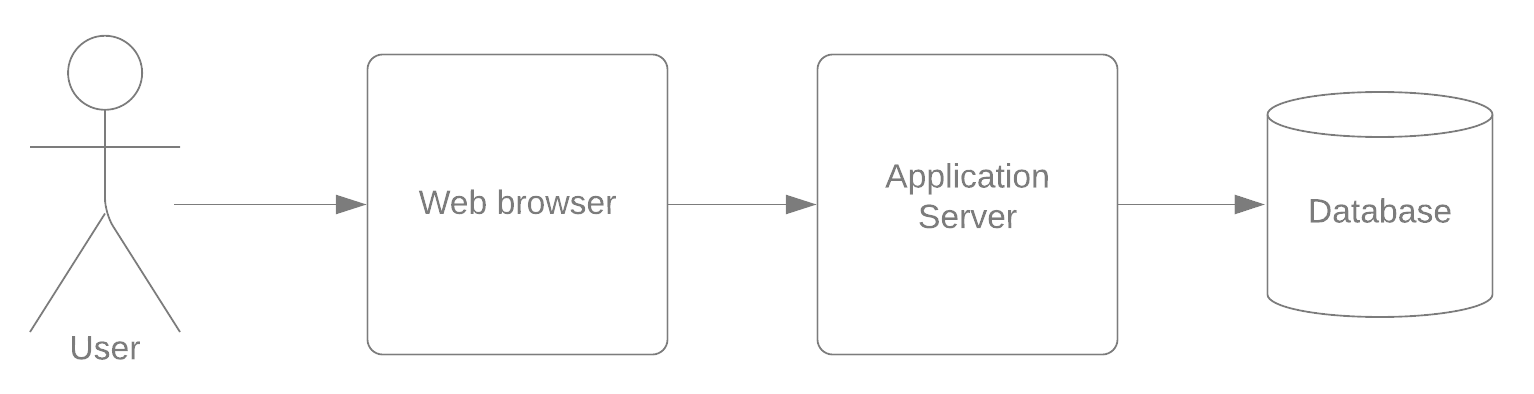
\includegraphics[width=\linewidth]{system_concept.png}
      \caption{Concept of the system}
      \label{fig:system_concept}
    \end{figure}

    User communicates with the system via web browser. 
    Web browser sends HTTP requests to the application server, which constructs the response using resources available in the database.

  \section{System architecture}
    \begin{figure}[h]
      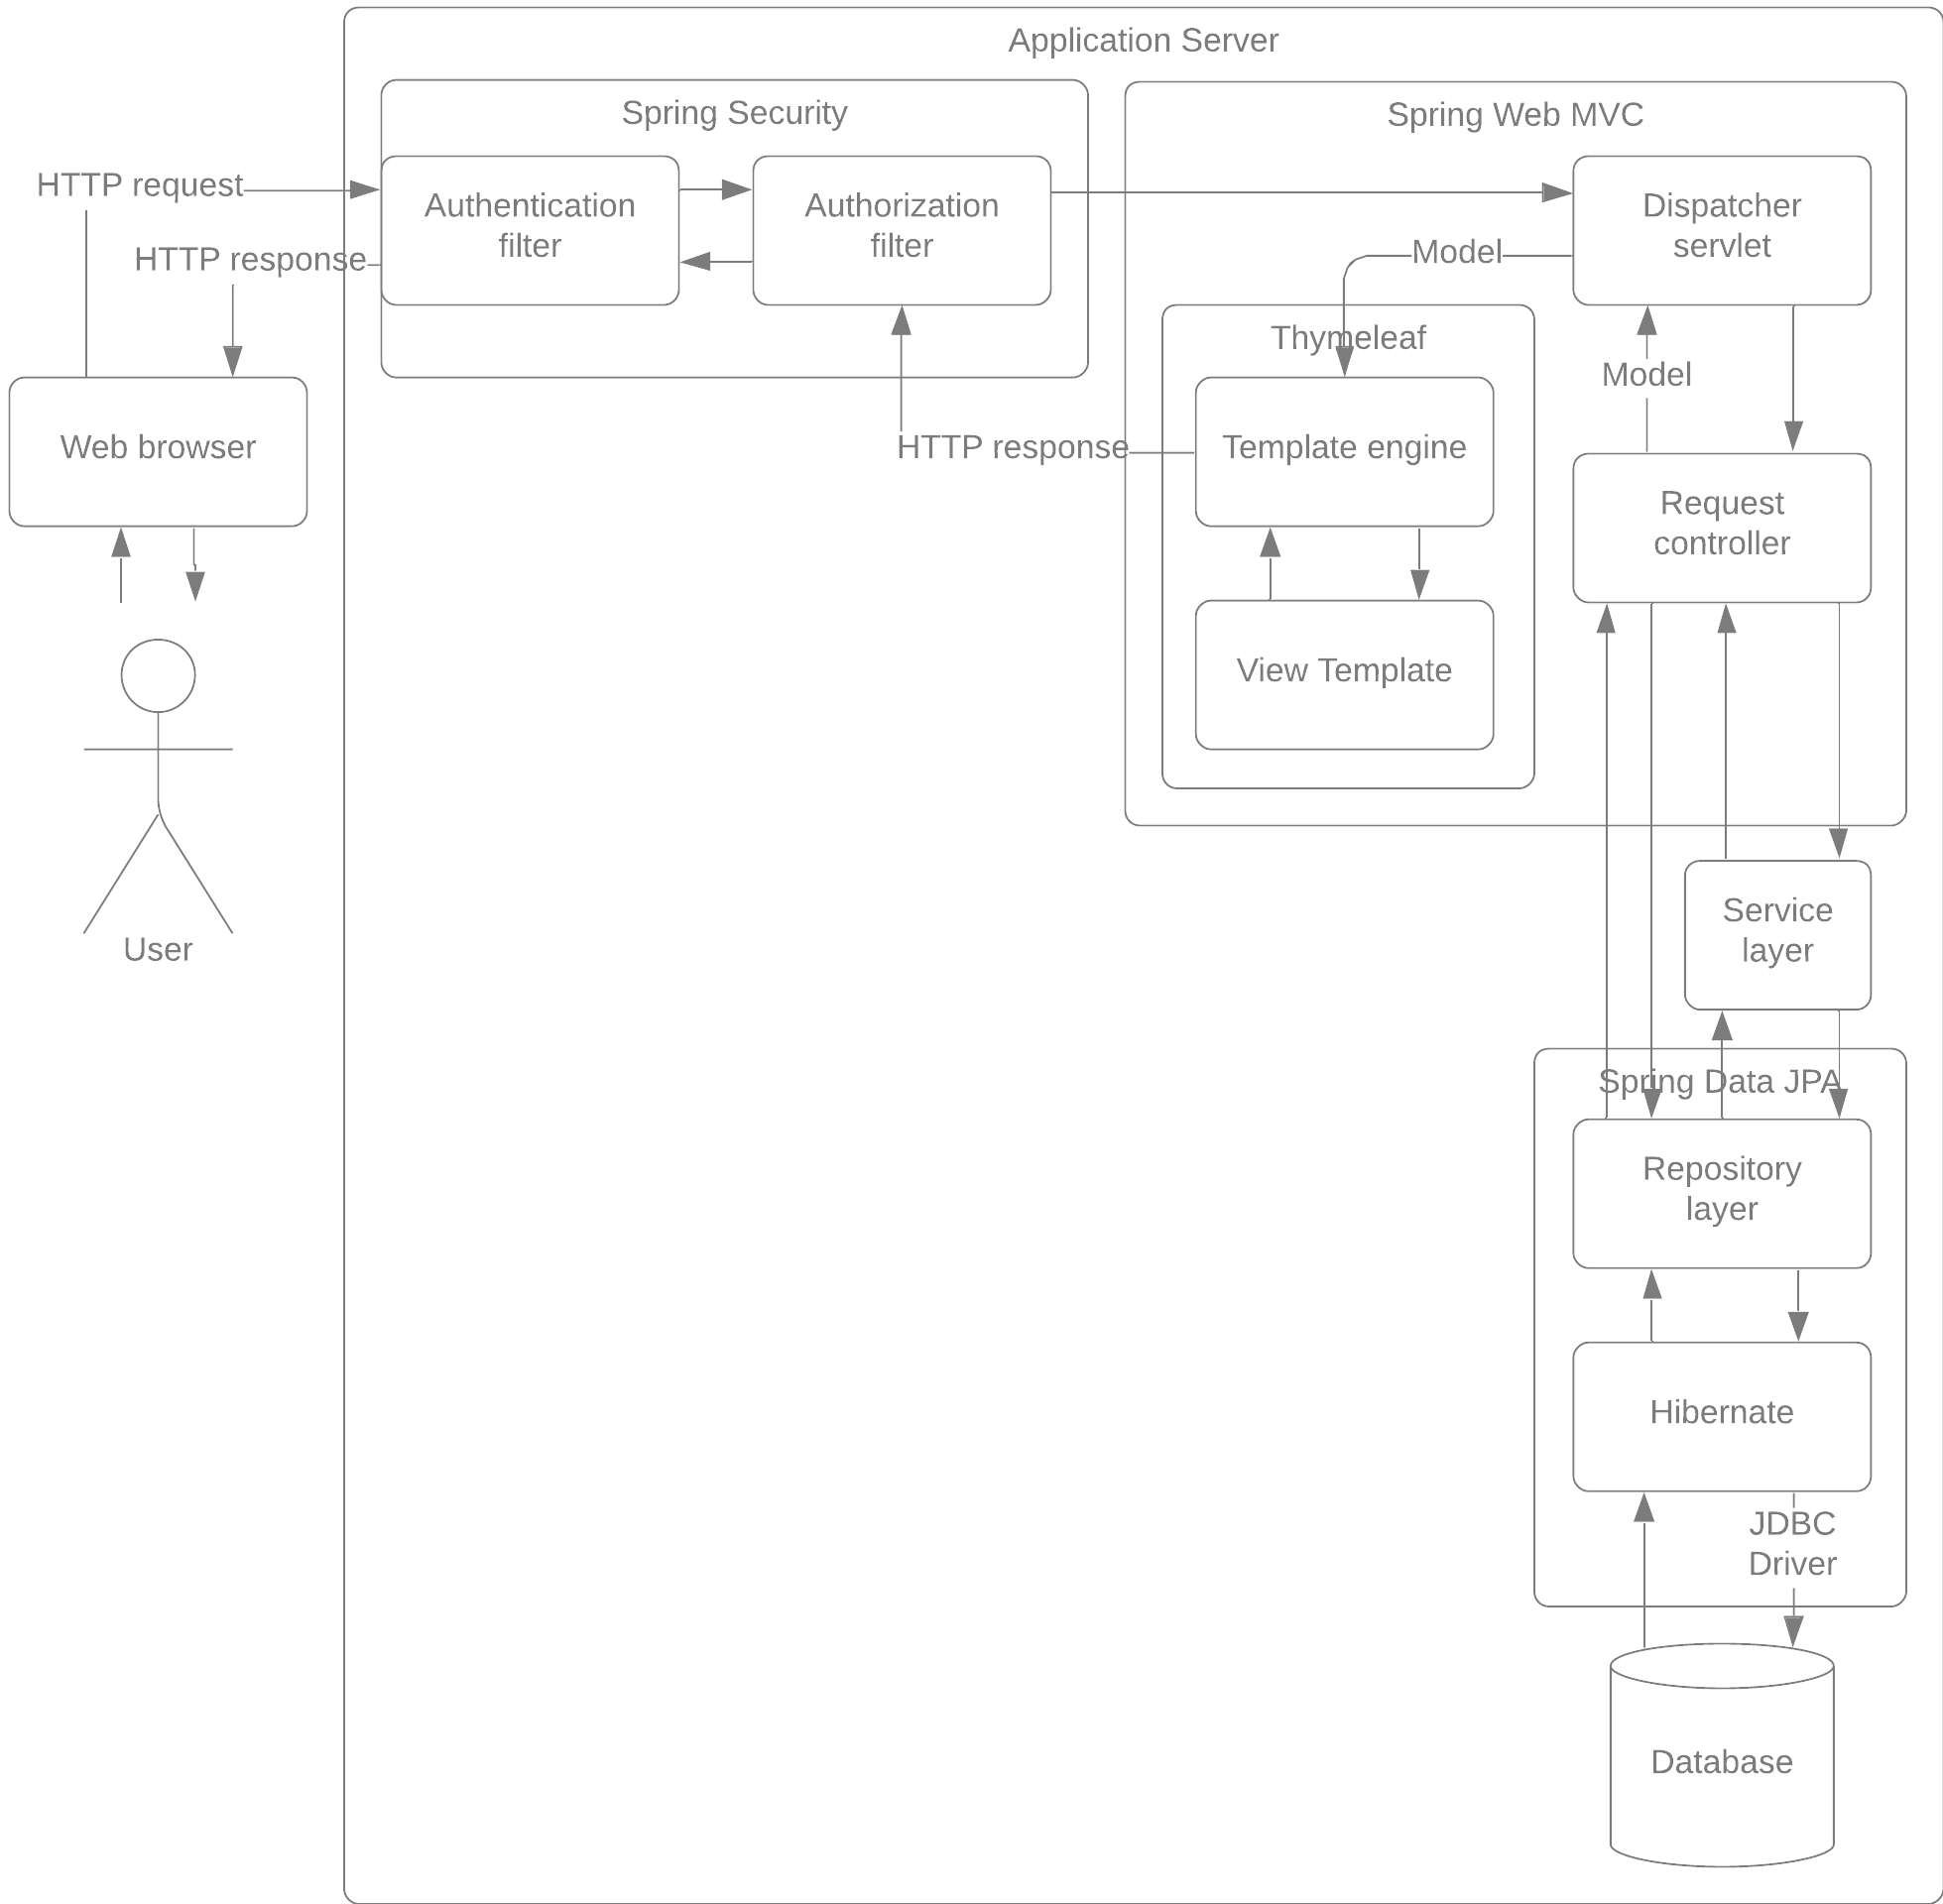
\includegraphics[width=\linewidth]{architecture_diagram.png}
      \caption{Application architecture}
      \label{fig:architecture_diagram}
    \end{figure}

    Figure \ref{fig:architecture_diagram} shows architecture of the application. 
    User interacts with web browser, and his actions trigger communication of the browser with application server via HTTP.
    Those requests are passed through security filters of Spring Security, which check if user is authenticated and authorized to fetch the resource he requests.
    After that, all requests hit dispatcher servlet, which delegates request to it's specific request controller.
    Repository layer provides data available directly in the database, 
    while service layer performs some additional logic, which is not available in the repository logic (some simple filtering of fetched data).
    Repository talks to database with help of Hibernate, JPA implementation used by Spring Data JPA. 
    Controller connects all data provided to it by service or repository layer into business logic, and constructs a view model for HTTP request.
    This view model is passed to template engine, 
    which applies this view model to specific view template (information regarding which template is also mentioned in view model), 
    and constructs HTTP response for this template.
    This response comes back to security filters, which send response back to web browser.
    \pagebreak

  \section{Data structure}
    \begin{figure}[h]
      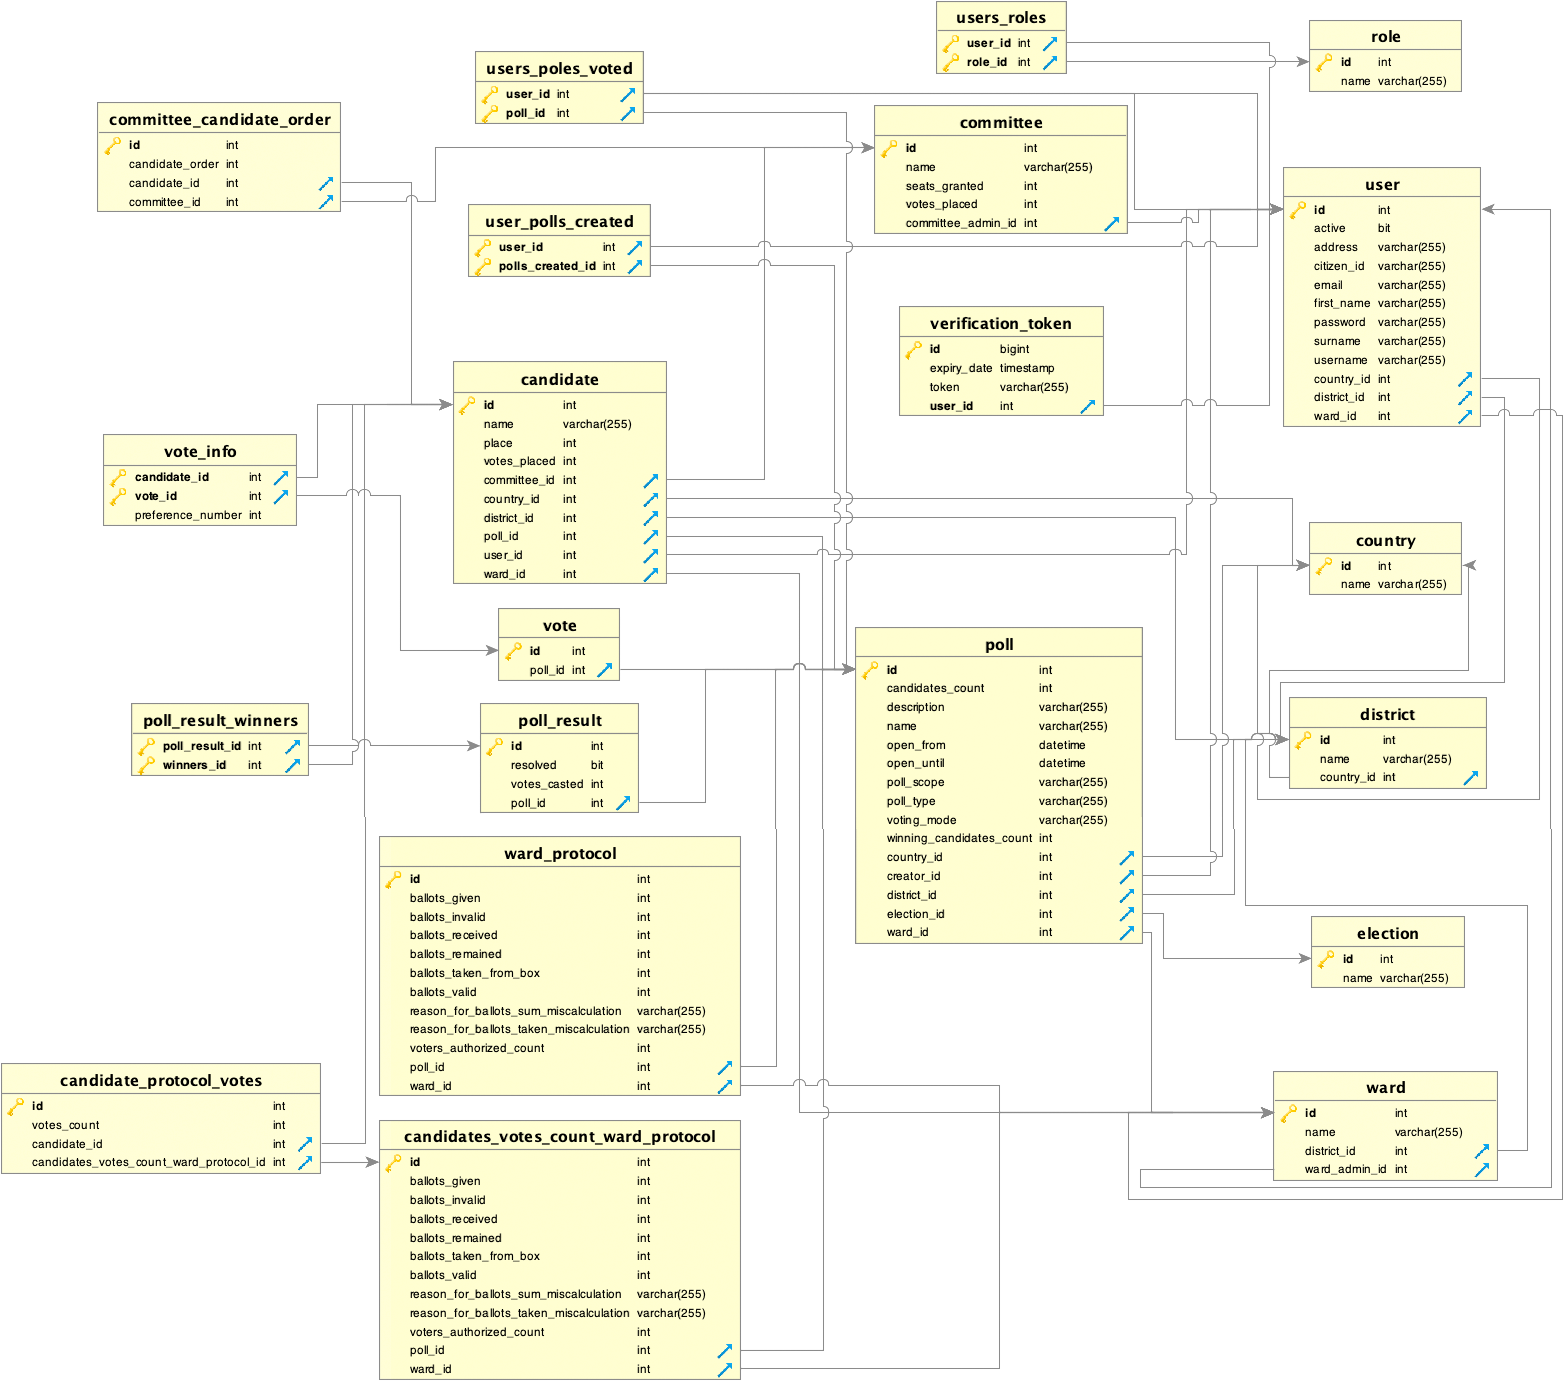
\includegraphics[width=\linewidth]{erd.png}
      \caption{Entity-Relationship Diagram}
      \label{fig:erd}
    \end{figure}

  \section{Implementation of the application}
    \subsection{Entity}
      An entity class is a representation of a table in a database.
      It can be treated as implementation of business data model, which is used to achieve some business result.

      On figure \ref{fig:ward_entity} we can see example code for an entity.
      Apart from standard Java syntax, there are some annotations related to JPA:
      \begin{itemize}
        \item @Entity---marks class as entity. It will be represented in database as a table.
        \item @Id---marks class field as primary key for table.
        \item @GeneratedValue---determines strategy for generating this value when writing to database in case of null.
        \item@ManyToOne---marks class field as many to one relationship with another entity. 
        It will store primary key of target entity in table of this entity.
        There is a twin annotation to this one, \lstinline|@OneToMany| for entity on the other side of this relation.
      \end{itemize}
    
    \subsection{Repository}
      A repository is an interface that allows a developer for interaction with objects stored in a database.
      Spring Data JPA provides out--of--the--box implementation of a CRUD repository.
      A \lstinline|@Repository| annotation allows Spring to identify such interface, create implementation of it and hold it in the context.
      It is easily extensible with help of custom finder methods, for example see figure \ref{fig:ward_repository} in the appendices.

    \subsection{Component}
      In order to help Spring identify dependency classes eligible for DI, we can annotate such classes with any derivative of \lstinline|@Component| annotation.
      When spring is scanning for components, \lstinline|@Component| annotated class will be treated as component, thus an object of such class will be created and held in the context.
      There are several derivatives of \lstinline|@Component| annotation, which serve the same purpose, but are named differently for simpler understanding of class role and behavior.
      Examples of \lstinline|@Component| specialized annotations:
      \begin{itemize}
        \item @Service
        \item @Controller
        \item @Repository
      \end{itemize}
      If needed, those dependencies can be injected using \lstinline|@Autowired| annotation.
      It looks for dependency of matching type as field under annotation, and assigns desired object to class field after owner object construction.
      Example of \lstinline|@Service| annotated class can be seen on figure \ref{fig:ward_service} in the appendices.

    \subsection{Controller}
      A controller is a class that can process HTTP requests. It is annotated with \lstinline|@Controller| annotation, along with \lstinline|@RequestMapping| annotation, 
      which value determines what URL this controller responds to.
      As HTTP has few methods that determine type of request under certain URL, controller class method annotations like \lstinline|@GetMapping| and \lstinline|@PostMapping|
      map HTTP method to class method, which that request triggers.

      There are many arguments that mapping method can take that give developers additional tools for processing HTTP request.
      This application uses \lstinline|Model| class as method argument to create a model passed to template.
      In case of POST HTTP method, we can use \lstinline|BindingResult| class in method argument to get information about form that was sent with HTTP request.
      Controller decides which template should be used by returning template location in \lstinline|String| type.
      This location is relative to folder \lstinline[language=bash]|APP_ROOT/src/main/resources/templates| by default.
      An example of Controller class can be seen on figure \ref{fig:ward_creation_controller} in the appendices.

    \subsection{View template}
      A view template is a HTML file with additional tags and attributes which are parsed by Thymeleaf after populating template with a model.
      This means that any errors in template file are runtime error, as template is parsed at the end of HTTP response generation flow \ref{fig:architecture_diagram}.

  \section{Applied design patterns}
    While many design patterns may be useful in big projects, there was no need to introduce any sophisticated methods of organizing application layers and communication.
    I kept it simple, and it worked for me. Here are two design patterns visible directly in the application code:
    \begin{itemize}
      \item MVC
      \item DI
    \end{itemize}

\chapter{Verification and validation}

\begin{itemize}
\item 
\end{itemize}

 
 
\chapter{Conclusions}

\begin{itemize}
\item 
\end{itemize}

 


%%%%%%%%%%%%%%%%%%%%%%%%%%%%%%%%%%%%%%%%%%
\backmatter
\pagenumbering{Roman}
\stepcounter{PagesWithoutNumbers}
\setcounter{page}{\value{PagesWithoutNumbers}}

\pagestyle{onlyPageNumbers}

%%%%%%%%%%% bibliography %%%%%%%%%%%%
\bibliographystyle{plain}
\bibliography{thesis}

%%%%%%%%%  appendices %%%%%%%%%%%%%%%%%%% 

\begin{appendices} 

\chapter*{List of abbreviations and symbols}

\begin{itemize}
  \item[API] Application Programming Interface
  \item[APP\_ROOT] Root directory of ballotbox project (with pom.xml file)
  \item[CRUD] Create, Read, Update, and Delete 
  \item[DI] Dependency Injection 
  \item[HOST] IP of host machine of application server  
  \item[HTML] HyperText Markup Language
  \item[HTTP] HyperText Transfer Protocol
  \item[JPA] Java Persistence API
  \item[JSP] JavaServer Pages
  \item[MVC] Model--View--Controller
  \item[PORT] Port on which application server listens
  \item[REST] Representational State Transfer
  \item[UML] Unified Modeling Language
  \item[URL] Uniform Resource Locator
\end{itemize}


\chapter*{Listings}
\begin{figure}
  \centering
    \begin{lstlisting}
//TODO: change root package name
package com.drzewo97.ballotbox.core.model.ward;

import com.drzewo97.ballotbox.core.model.candidate.Candidate;
import com.drzewo97.ballotbox.core.model.district.District;
import com.drzewo97.ballotbox.core.model.user.User;

import javax.persistence.*;
import java.util.Set;

@Entity
public class Ward {
          
@Id
@GeneratedValue(strategy = GenerationType.IDENTITY)
private Integer id;
          
private String name;
          
@ManyToOne
private District district;
          
@OneToMany(mappedBy = "ward")
private Set<Candidate> candidates;
          
@ManyToOne
private User wardAdmin;

...

get methods
set methods
}
    \end{lstlisting}
    \caption{The \lstinline|Ward| entity.}
    \label{fig:ward_entity}
  \end{figure}

  \begin{figure}
    \centering
    \begin{lstlisting}
package com.drzewo97.ballotbox.core.model.ward;

import com.drzewo97.ballotbox.core.model.country.Country;
import com.drzewo97.ballotbox.core.model.district.District;
import org.springframework.data.repository.CrudRepository;
    
import java.util.Set;
    
public interface WardRepository extends CrudRepository<Ward, Integer> {
  Boolean existsByNameAndDistrict_Name(String name, String districtName);
  Set<Ward> findAllByWardAdminIsNull();
  Set<Ward> findAllByWardAdminUsername(String username);
  Set<Ward> findAllByDistrict(District district);
  Set<Ward> findAllByDistrictCountry(Country country);
}
    \end{lstlisting}
    \caption{The \lstinline|Ward repository|.}
    \label{fig:ward_repository}
  \end{figure}

  \begin{figure}
    \centering
    \begin{lstlisting}
package com.drzewo97.ballotbox.core.service.ward;

import com.drzewo97.ballotbox.core.model.poll.Poll;
import com.drzewo97.ballotbox.core.model.ward.Ward;
import com.drzewo97.ballotbox.core.model.ward.WardRepository;
import org.springframework.beans.factory.annotation.Autowired;
import org.springframework.stereotype.Service;
  
import java.util.HashSet;
import java.util.Set;
  
@Service
public class WardServiceImpl implements WardService {
    
  @Autowired
  private WardRepository wardRepository;
   
  @Override
  public Boolean isWardAdmin(String username, Integer wardId) {
    Set<Ward> adminsWards = wardRepository.findAllByWardAdminUsername(username);
    return adminsWards.stream().filter(ward -> ward.getId().equals(wardId)).count() > 0;
  }
    
  /**
   * Get all wards that could and should provide protocols for this poll
   * @param poll
   * @return
   */
  @Override
  public Set<Ward> findAllEligibleForPollProtocol(Poll poll) {
    Set<Ward> returner = new HashSet<>();
      
    switch (poll.getPollScope()){
      case COUNTRY:
        returner.addAll(wardRepository.findAllByDistrictCountry(poll.getCountry()));
        break;
      case DISTRICT:
        returner.addAll(wardRepository.findAllByDistrict(poll.getDistrict()));
        break;
      case WARD:
        returner.add(poll.getWard());
        break;
    }
      
    return returner;
  }
}
    \end{lstlisting}
    \caption{The \lstinline|Ward service|.}
    \label{fig:ward_service}
  \end{figure}

  \begin{figure}
    \centering
    \begin{lstlisting}
import org.springframework.web.bind.annotation.ModelAttribute;
import org.springframework.web.bind.annotation.PostMapping;
import org.springframework.web.bind.annotation.RequestMapping;
          
import java.util.stream.Collectors;
import java.util.stream.StreamSupport;
          
@Controller
@RequestMapping(path = "/panel/ward/create")
public class WardCreationController {
  @Autowired
  private WardRepository wardRepository;
            
  @Autowired
  private DistrictRepository districtRepository;
            
  @ModelAttribute("ward")
  private Ward ward() {
    return new Ward();
  }
            
  @GetMapping
  private String showWardCreate(Model model){
    model.addAttribute("districts", StreamSupport.stream(districtRepository.findAll().spliterator(), false).collect(Collectors.toList()));
    return "panel/ward_create";
  }
            
  @PostMapping
  private String createWard(@ModelAttribute("ward") Ward ward, BindingResult result){
    if(wardRepository.existsByNameAndDistrict_Name(ward.getName(), ward.getDistrict().getName())){
      result.rejectValue("name", "name.exist", "Ward already exists.");
    }
              
    if(result.hasErrors()){
      return "panel/ward_create";
    }
              
    wardRepository.save(ward);
              
    return "redirect:create?success";
  }
}
    \end{lstlisting}
    \caption{The \lstinline|Ward creation controller|.}
    \label{fig:ward_creation_controller}
  \end{figure}

\chapter*{Contents of attached CD}

The thesis is accompanied by a CD containing:
\begin{itemize}
\item thesis (\LaTeX\ source files and final \texttt{pdf} file),
\item source code of the application,
\item test data.
\end{itemize}
 

\listoffigures
\listoftables
	
\end{appendices}


\end{document}


%% Finis coronat opus.